%%%%%%%%%%%%%%%%%%%%  練習問題（旧 prob_p2.png / prob_p3.png / prob_p4.png）  %%%%%%%%%%%%%%%%%%%%
\Rank{A問題}

\Mon{基本事項の確認}

以下の設問に答えよ．
\begin{komon}
\ko{1} $200\U{m}$進むのに$5\U{s}$かかったときの平均の速さは何$\U{m/s}$か．
\ko{2} 直線道路を速度$5.0\U{m/s}$で走っていた自動車がある時刻に加速し始め，$8.0\U{s}$後に速度$13\U{m/s}$になった．この間の平均の加速度は何$\U{m/s^2}$か．
\ko{3} 直線上を初速度$3.0\U{m/s}$，加速度$0.20\U{m/s^2}$で運動している物体がある．加速し始めてから$5.0\U{s}$後のこの物体の速さは何$\U{m/s}$か．また，この間の移動距離は何$\U{m}$か．
\ko{4} 直線上を速度$20\U{m/s}$で走っていた自動車がブレーキをかけたところ，$10\U{m}$だけ等加速度直線運動をして止まった．ブレーキをかけてから止まるまでの加速度は何$\U{m/s^2}$か．
\ko{5} 東向きに速度$5\U{m/s}$で進む船の甲板上で，北向きに速度$5\U{m/s}$で走る人は，海面に対してどちらの向きに何$\U{m/s}$の速さで進んでいるか．
\ko{6} ロケットが仰角$60^\circ$の向きに速さ$200\U{m/s}$で飛んでいる．ロケットの速度の水平成分と鉛直成分は何$\U{m/s}$か．
\ko{7} 速度$10\U{m/s}$で走っている列車から，線路に平行な道路を同じ向きに速度$40\U{m/s}$で走っている自動車を見ると，どちら向きに何$\U{m/s}$で走っているように見えるか．
\end{komon}

\Rank{B問題}

\Mon{平均の速度と瞬間の速度}

\hspace{1zw}$x$軸上を運動する物体の時刻$t\U{s}$における座標$x\U{m}$が$x(t)=5t^2-16t+10$で与えられている．
\begin{komon}
\ko{1} 時刻$2\U{s}$から$3\U{s}$の間のこの物体の平均の速度を求めよ．
\ko{2} 時刻$2\U{s}$における瞬間の速度を求めよ．
\ko{3} 任意の時刻$t\U{s}$におけるこの物体の速度を求めよ．
\end{komon}

\newpage

\Mon{$v-t$グラフ}\Sitei

\begin{zuright}{48mm}
\hspace{1zw}右図は直線上を運動する物体の時刻$t\U{s}$と速度$v\U{m/s}$の関係を示したグラフである．
\begin{komon}
\ko{1} 時刻$0\U{s}$から$2.0\U{s}$の間の加速度を求めよ．
\ko{2} 時刻$6.0\U{s}$から$10.0\U{s}$の間の加速度を求めよ．
\ko{3} 動き始めてから静止するまでに動いた距離を求めよ．
\ko{4} 加速度と時刻の関係を表すグラフを描け．
\end{komon}
\zusep
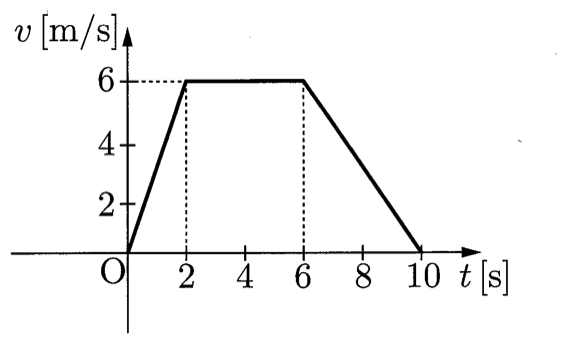
\includegraphics[keepaspectratio,width=48mm]{fig/ch1_p3_vt.png}
\end{zuright}

\Mon{等加速度直線運動}

\hspace{1zw}直線道路上を速さ$10\U{m/s}$で走っていた自動車が一定の割合で加速し，$5.0\U{s}$後には速さ$16\U{m/s}$となった．
\begin{komon}
\ko{1} この間の加速度を求めよ．
\ko{2} この間の移動距離を求めよ．
\end{komon}
\hspace{1zw}次に，同じ直線道路上を速さ$16\U{m/s}$で走っていたこの自動車が一定の割合で減速し，$80\U{m}$だけ走って停止した．
\begin{komon}
\ko{3} この間の加速度を求めよ．
\ko{4} 減速し始めてから停止するまでに要した時間を求めよ．
\end{komon}

\Mon{相対速度}\Sitei

\begin{zuright}{43mm}
\hspace{1zw}右図のように船$\mathrm{A}$は東向きに速さ$5.0\U{m/s}$，船$\mathrm{B}$は北向きに速さ$5.0\U{m/s}$，船$\mathrm{C}$は西向きに速さ$5.0\U{m/s}$で，それぞれ海面上を進んでいる．
\begin{komon}
\ko{1} $\mathrm{C}$から見た$\mathrm{A}$の相対速度の大きさと向きを求めよ．
\ko{2} $\mathrm{B}$から見た$\mathrm{A}$の相対速度の大きさと向きを求めよ．
\end{komon}
\zusep
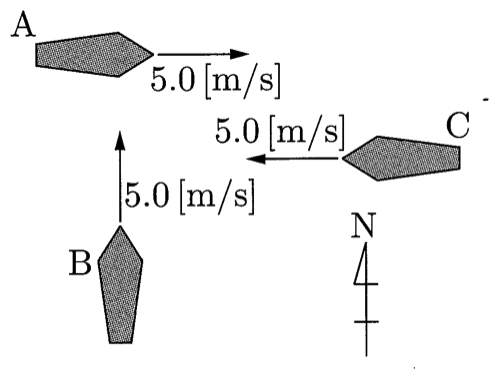
\includegraphics[keepaspectratio,width=43mm]{fig/ch1_p3_boat.png}
\end{zuright}

\Mon{速度の合成}

\begin{zuright}{41mm}
\hspace{1zw}静水上を速さ$10\U{m/s}$で進むことのできる船が，右図のように流れの速さ$6.0\U{m/s}$，川幅$100\U{m}$の川を横断する．
\begin{komon}
\ko{1} 船が岸に対して直角に進むとき，岸に対する船の速さを求めよ．
\ko{2} (1)のとき，船が川を横断するのに要する時間を求めよ．
\ko{3} 船が最も短い時間で川を横断するとき，船が対岸に着くまでに下流に流される距離を求めよ．
\end{komon}
\zusep
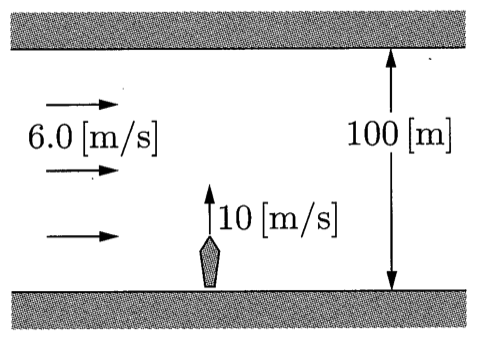
\includegraphics[keepaspectratio,width=41mm]{fig/ch1_p3_river.png}
\end{zuright}

\Rank{C問題}

\Mon{等加速度直線運動}

\hspace{1zw}一直線上を右向きに速さ$4.0\U{m/s}$で進んでいた物体がある時刻に等加速度運動をし始めたところ，$8.0\U{s}$後には左向きに速さ$12.0\U{m/s}$となった．等加速度運動をし始めた時刻を$0\U{s}$として，以下の問いに答えよ．
\begin{komon}
\ko{1} 加速度の大きさと向きを求めよ．
\ko{2} 右向きを正として，時刻$t\U{s}$における物体の速度$v(t)\U{m/s}$を求めよ．
\ko{3} 物体が出発点から右に最も離れる時刻を求めよ．
\ko{4} 物体が出発点を左向きに通過するときの速さを求めよ．
\ko{5} 時刻$8.0\U{s}$における出発点から物体の位置を求めよ．
\end{komon}

\newpage

\Mon{$v-t$グラフ}

\begin{zuright}{63mm}
\hspace{1zw}右図は，$x$軸上の原点を時刻$0\U{s}$に出発した物体の，速度$v\U{m/s}$と時刻$t\U{s}$の関係を示している．
\begin{komon}
\ko{1} 時刻$t\U{s}$における物体の加速度を求めよ．
\ko{2} 時刻$9\U{s}$における物体の$x$座標を求めよ．
\ko{3} 時刻$13\U{s}$における物体の$x$座標を求めよ．
\ko{4} 時刻$0\U{s}$から$13\U{s}$の間に物体が動いた道のりを求めよ．
\end{komon}
\zusep
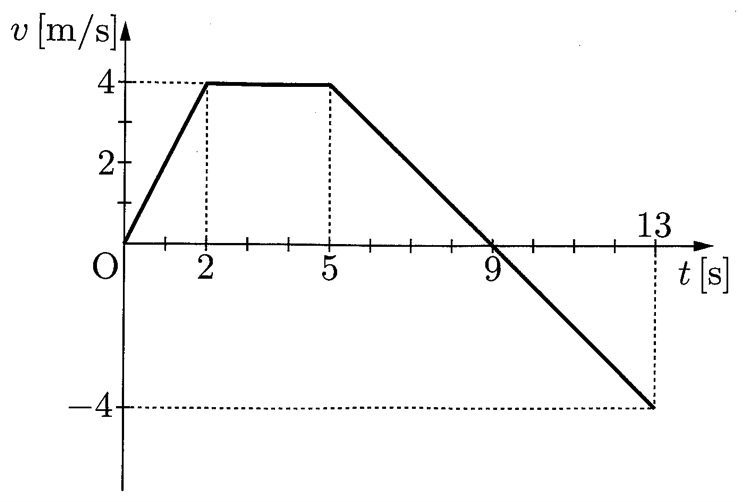
\includegraphics[keepaspectratio,width=63mm]{fig/ch1_p4_vt.png}
\end{zuright}
